\documentclass[11pt]{jreport}
\usepackage[dvipdfmx, hiresbb]{graphicx}
\usepackage[top=30truemm, bottom=30truemm, left=30truemm, right=30truemm]{geometry}
\usepackage{float}
\usepackage{ascmac}
\usepackage{amsmath}
\usepackage{amssymb}
\usepackage{bm}
\usepackage{amsfonts}
\usepackage{here}
\begin{document}
\title{Contest\\}
\author{東京理科大学工学部経営工学研究科\\新田 翔 \and 東京理科大学工学部第一部経営工学科\\黒木 裕鷹}
\maketitle
\begin{abstract}

\end{abstract}


\chapter{ルールに基づいた戦略の決定}
\section{ルールの概観}

本コンテストで行うシミュレーションは一般的に行われている金融取引とは異なる.最終的な目標は一定のルールのもとでより高い収益を獲得することであるため,投資の戦略もルールに基づいたものでなくてはならない.ルールを概観し,以下にまとめた.

\begin{enumerate}
\item ルール
\begin{enumerate}
\item ポートフォリオ登録時点で時価総額が1億円以内になるように登録
\item 10銘柄以上、30銘柄以下でのポートフォリオを構成
\item 2017年7月31日までであれば1度だけ銘柄の入れ替え(リバランス)が可能
\item ロングポジションのみ(空売り禁止)
\item 手数料は考慮しない
\end{enumerate}

\item パフォーマンス計測期間
\begin{enumerate}
\item  2017年7月3日 $\sim$ 2017年8月31日
\end{enumerate}

\item パフォーマンス測定方法
\begin{enumerate}
\item ポートフォリオ機能「トータルリターン(\%)」を頻度日次・円建てで計測
\item ポートフォリオ登録は登録日より2営業日前の終値をコスト価格として登録
\item ポートフォリオ登録後、6月中の価格変動による時価総額の増減を含め7月3日から8月31日の間でパフォーマンスを計測
\end{enumerate}
\end{enumerate}

以上のルールの中で,時間的な制約は1-c, 2-aである.これらにより1か月単位のバイアンドホールドを強いられ,さらにルール3-bにより裁定機会が失われることになる.つまり,金融資産の価格変動は何を根拠として起こっているのか,という視点で考える必要があり,それに基づいて価格が上昇する銘柄を追い求めていくことになる.次の1.2節では,価格変動の源泉について考察した.

\section{価格変動の源泉}
金融資産は一般的な商品と異なり、投資目的やリスクヘッジ目的で購入されることがほとんどであるから,その価格は需要供給の関係だけでなく将来の見通しにも影響される。つまり、「情報」が価格に織り込まれるのである。すると、未だ織り込まれていない「情報」を見つけ出して特定の銘柄を購入し、織り込まれた時点で売却する、という戦略が考えられる。この手法は一見有効であるように思えるが、ここには一つ盲点ある。それは、証券アナリストや裁定取引を行う投資家をはじめとする高度に習熟したプロフェッショナルの存在である。習熟したプロ達はいち早く織り込まれていない情報を日々見つけ出し、ポートフォリオに組み込むことを目標にしている。アナリスト達が織り込んでいない情報を見つけ出す手段として、アナリスト達が注目していない、またはポートフォリオに組み込めないような市場や超小型銘柄に焦点を当てる方向が考えられる。しかしルール1-c, 2-a, 3-bの存在により、この手法も困難であることが分かる。織り込まれていない情報が織り込まれたとして、8月31日までその価格が継続する可能性や測定期間内にその情報が織り込まれる可能性が高くないからだ。またリバランスを行うことにより利益を確定させても,その先1か月以上で同様のリスクを背負わなくてはならない.

織り込まれていない「情報」に着目するような投資戦略を避けるとすれば,他にどのようなアプローチが考えられるだろうか.次の1.3節では別の見方から価格変動を眺める.
 
\section{価格変動の共通要因}
世界には無数の企業があり,それぞれが異なった性質を持っている.
持っている技術やリリースしている商品,組織体系などが多種多様であるということだ.
しかし,複数の企業に共通している性質も考えられる.
例えば所属国や業種,企業の規模などだ.
このような共通の要因のうち,株価の変動に関係を持つものも当然存在するだろう.
FamaとFrenchは米市場における実証分析を行い,企業規模(size)や簿価比時価率(Value)が株価の収益構造に関与していると結論付けた.
つまり,企業規模の小さい銘柄や,時価総額が総資産額に比べて割安な銘柄は平均的に高い収益を見せるということだ.
この現象はそれぞれ小型株効果,バリュー株効果と呼ばれ,代表的なアノマリーとして認識されている.
先ほどのモデルはFama-Frenchの3ファクターモデルと呼ばれ,両者はその功績により2013年にノーベル経済学賞を受賞した.
実際に似たような性質(業種や企業規模など)の銘柄は似たような価格変動を見せることが多く,FamaとFrenchが対象とした米市場に限らず,金融資産の価格変動が共通の要因に影響されているという主張は自然なものだと考えられる.

このような価格変動の共通要因の存在は,平均的にリターンを得る投資戦略の足掛かりとなるのではないだろうか.

\section{様々な理論}
資産価格変動の共通要因を考えた理論として最も広く知られているのはウィリアム・シャープらによる資本資産価格モデル(capital asset pricing model : CAPM)だろう.
市場ポートフォリオを唯一の共通要因とした資産価格の評価手法である.
CAPMは1960年代より不動の地位を築き,その計算の簡便さもあり現在でも広く用いられている.
しかし1970年代以降,CAPMに対する様々な批判や問題点が提起され,代わりとなる新たな理論が提唱され続けてきた.
2章で触れるが,CAPMが必要とする仮定が非常に限定的であり,到底成立するものではない,という主張である.
そこで,本コンテストではより確からしい共通要因を考えるため,独自のマルチ・ファクターモデルを構築することとした.

詳細については後に触れるが,APTはCAPMと異なり,全資産の収益の同時分布が正規分布であることを必要しないのである.
また,これも後述するが,APTはファクターモデルの基礎と捉えることが出来る.

\section{戦略の決定}
1.2節で述べたように、これから価格に織り込まれる「情報」を追うのではなく違う視点から戦略を決定する必要がある.
また1.3節で述べた,Fama-Frenchの3ファクターモデルをはじめとするマルチ・ファクターモデルにより,CAPMよりも確からしい資産の価格変動の構造を考えることができる.
そこで独自のマルチ・ファクターモデルを構築し,「直近で平均的に勝てている投資スタイル」を見つけ出すことが出来れば2ヶ月間の収益を競う本コンテストにおいても成果を上げることが出来るのではないかと考えた.
なお,本コンテストは2カ月間のみの短いものであり,偶発的な金融危機については考えないこととする.
とはいえ,収益に見合わないリスクを持つポートフォリオを構成することには何の利点も考えられないため,特に理由がない限り構成銘柄数は最大の30銘柄を考える.

市場には無数の裁定取引を行う投資家が存在すること,さらにコンテストのルールにより,鞘取りに関しては全く行うことが出来ない.
市場に裁定機会が存在しないことを主な仮定とするAPTと非常に相性の良いものであり,本コンテストのルールの下で収益を出すために十分有用であると考えられる.

マルチ・ファクターモデルにより各銘柄の収益構造を推定した後の問題はポートフォリオに組み込む資産をどのように選択するかである.
投資には必ずリスクが伴い,投資家はそのリスクを代償にリターンを求める.
そこでここでは,それぞれのファクターの持つリスクに晒される「価値」を考えることとした.
この「価値」は通常リスク・プレミアムと呼ばれる.高いリスク・プレミアムを持つファクターに対してリスクを取り,低いリスク・プレミアムを持つファクターに対して分散化することを考えていく.


\chapter{理論}
\section{シングル・ファクターモデルとしてのCAPM}
CAPMの枠組みにおいて,金融資産$i$の収益率$r_i$は唯一の共通要因である市場ポートフォリオの収益率$R_M$に依存する変動と資産特有の変動$\varepsilon_i$に分けられ,以下のように表される.また,$\varepsilon_i$は資産間で相互に無相関であると仮定される.$r_f$は無リスク利子率を表す定数であり,信用の高い長期国債の年利が一般的に用られる.
\begin{equation}
\begin{split}
&r_i - r_f = \alpha_i + \beta_i(R_M - r_f) + \varepsilon_i\\
&\varepsilon_i \sim i.i.d.N(0,\sigma_i^2)\\
&Cov(R_M, \varepsilon_i) = 0\\
&Cov(r_i, r_j) = 0 \qquad (i \neq j)
\label{eq:CAPM}
\end{split}
\end{equation}
ここで,$\beta_i$は金融資産$i$の市場ポートフォリオへの感度を表し,$\alpha_i$は市場ポートフォリオに対する期待超過収益率を表している.式(\ref{eq:CAPM})より$r_i$の分散を求めると
\begin{equation}
Var(r_i) = \beta_i^2Var(R_M) + Var(\varepsilon_i) \qquad (\text{∵}Cov(R_M, \varepsilon_i) = 0)
\label{eq:CAPM_var}
\end{equation}
となり,この右辺第1項はシステマティック・リスクと呼ばれ,シングル・ファクターであるマーケットの動きにより説明可能な部分である.
また右辺第2項はマーケットに依存しないアンシステマティック・リスクと呼ばれる.
これらのリスクのうち,アンシステマティック・リスクはポートフォリオ選択によって除去可能であるとしばしば言われる.

次に式(\ref{eq:CAPM})により記述される資産で構成したポートフォリオを考える.市場を構成する資産数を$N$とすると,資産$i(i=1,\cdots,N)$の保有比率が$w_i$であるようなポートフォリオ$P$の収益率$R_P$は以下で与えられることになる.
\begin{equation}
\begin{split}
R_P &= \alpha_P + \beta_PR_M + \varepsilon_P\\
&= \sum_{i=1}^N w_i\alpha_i
+\left(\sum_{i=1}^N w_i\beta_i\right)R_M
+\sum_{i=1}^N w_i\varepsilon_i
\end{split}
\end{equation}
また,このポートフォリオの分散は以下で与えられる.
\begin{equation}
\begin{split}
Var(R_P) &= \beta_P^2 Var(R_M) + Var(\varepsilon_P)\\
& = \left(\sum_{i=1}^N w_i\beta_i\right)^2Var(R_M) + \sum_{i=1}^N w_i^2 Var(\varepsilon_i)
\end{split}
\end{equation}
この$\beta_P$がポートフォリオの市場ポートフォリオに対する感度になり,$\alpha_P$がポートフォリオの市場ポートフォリオに対する期待超過収益率となる.




\section{CAPMに対する批判}
1.4節で述べたように,CAPMに対しては様々な批判が為され,実証分析が行われてきた.以下にその代表的なものを挙げる.
\begin{itemize}
\item Basu(1977)\\
ニューヨーク証券取引所において,PERの低い銘柄が高い銘柄に比べて良いパフォーマンスを見せることを実証した.
\item Rolf Banz(1981)\\
企業規模の小さい銘柄が大きい銘柄に比べて良いパフォーマンスを見せることを実証した.
\item Jagadeesh, Titman(1993)\\
モメンタムの強い銘柄が市場をけん引し続ける傾向があることを実証した.
\end{itemize}

式(\ref{eq:CAPM_var})の第2項であるアンシステマティック・リスクはポートフォリオ選択によって除去可能であると言われてきたが,これが不可能であることをいずれの研究も示している.企業特有の$\varepsilon_i$が企業ごとに独立ではなく,共分散が存在しているということである.つまりこのことは,マーケットではない共通要因も存在し,それらがアノマリーの原因となっていることを示唆している.CAPMの枠組みでは,市場ポートフォリオによって説明できる部分(ベータ)と出来ない部分(アルファ)に分けられ,超過収益であるアルファはポートフォリオ・マネージャーの手腕によるものたと解釈された.しかし次節で述べるマルチ・ファクターモデルの発見により,マネージャーの手腕によると言える部分は徐々に減り,代わりにファクターのリスク・プレミアムによる部分が増えることとなった.以下の図\ref{fig:beta}にそのイメージ図を示した.

\begin{figure}[H]
	\begin{center}
		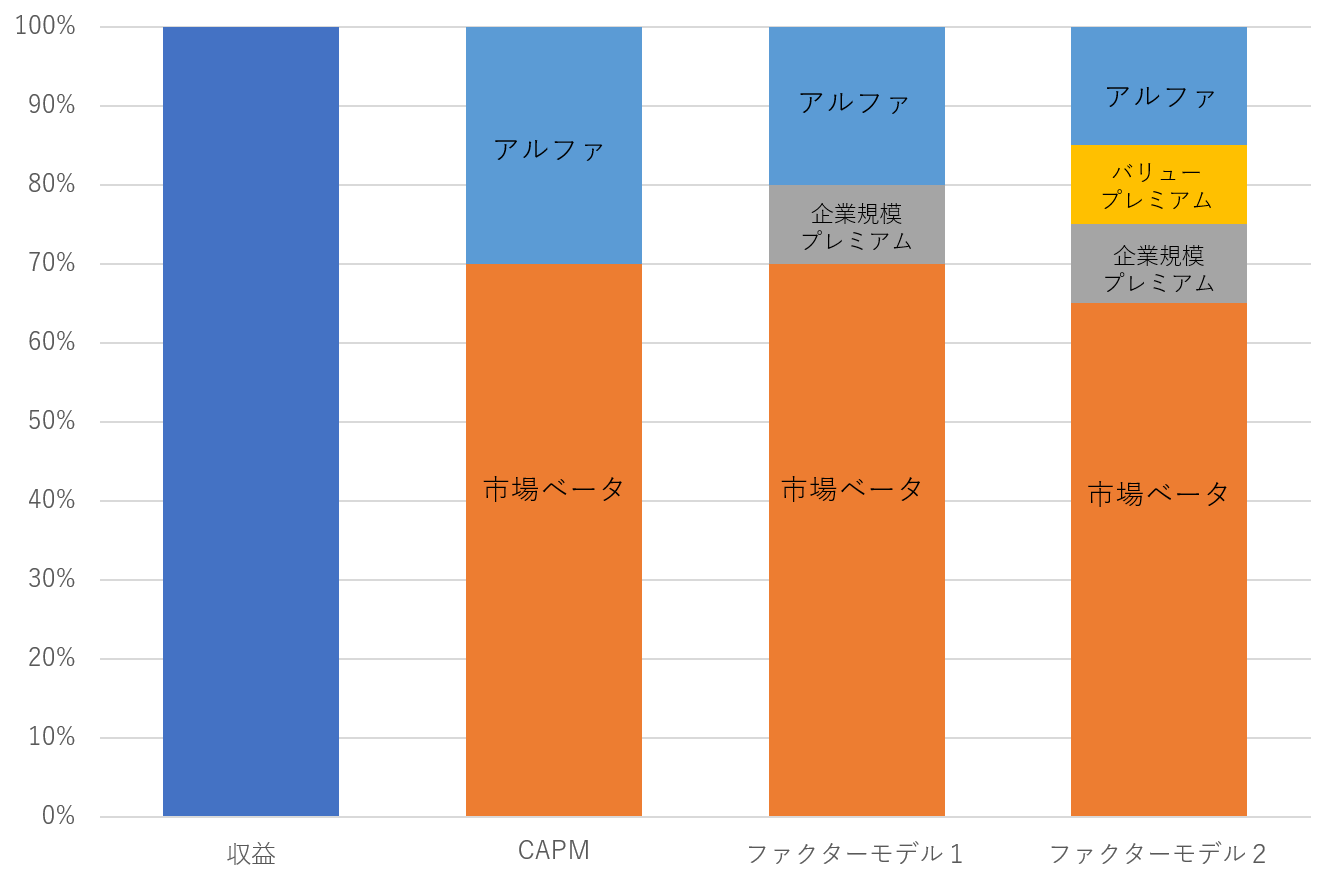
\includegraphics[width=14cm]{./fig/beta}
		\caption{ベータの移り変わり}
		\label{fig:beta}
	\end{center}
\end{figure}




\section{マルチ・ファクターモデル}
ここでは,各資産の収益率が$m$個の共通要因に依存するマルチ・ファクターモデルを考える.金融資産$i$の収益率$r_i$は企業特有の部分$\varepsilon_i$と共通要因であるファクター$F_k(k=1,\cdots,m)$によって決定される.また,$\varepsilon_i$は資産間で相互に無相関であると仮定すると,$r_i$は以下のように表される.
\begin{equation}
r_i = \alpha_i + \beta_{i,1}F_1 + \beta_{i,2}F_2 + \cdots + \beta_{i,k}F_k + \cdots + \beta_{i,N}F_m + \varepsilon_i
\end{equation}
ここで,2.1節と同様,資産$i(i=1,\cdots,N)$の保有比率が$w_i$であるようなポートフォリオ$P$の収益率$R_P$を考えると以下のようになる.
\begin{equation}
\begin{split}
R_P &= \alpha_P + \beta_{P,1} F_1 + \beta_{P,2} F_2 + \cdots + \beta_{P,m} F_m + \varepsilon_P\\
&=\sum_{i=1}^N \alpha_i + F_1 \sum_{i=1}^N w_i \beta_{i,1} + \cdots + F_m \sum_{i=1}^N w_i \beta_{i,m} + \sum_{i=1}^N w_i\varepsilon_i\\
&= \sum_{i=1}^N \alpha_i + \sum_{k=1}^m \sum_{i=1}^N w_i \beta_{i,k} F_k + \sum_{i=1}^N w_i\varepsilon_i
\label{eq:multi}
\end{split}
\end{equation}

%次に,式(\ref{eq:multi})の分散を考える.
%ポートフォリオの分散は求めたほうが良いの?
\section{Fama-Frenchの3ファクターモデル}
数あるマルチ・ファクターモデルのうち,最も知られているものはFama-Frenchの3ファクターモデルだろう.このモデルは市場ポートフォリオ,時価総額,簿価時価比率の3つをファクターとしている.数式としては,以下のように表されることが多い.
\begin{equation}
r_i - r_f = \beta_i^{MKT}(R_M - r_f) + \beta_i^{SMB}SMB + \beta_i^{HML}HML
\label{eq:fama-french}
\end{equation}
ここで,$r_f$は無リスク利子率であり,長期国債の年利が用いられることが多い.また$SMB$はSmall Minus Bigの略であり,時価総額下位50\%の時価総額加重平均ポートフォリオから上位50\%の時価総額加重平均ポートフォリオを引いたものである.つまり,企業規模の小さい銘柄が大きい銘柄に対して余剰に得ている収益を表すファクターである.次にHMLであるが,これはHigh Minus Lowの略であり,簿価時価比率上位30\%の時価総額加重ポートフォリオから下位30\%の時価総額加重ポートフォリオを引いたものである.つまり,総資産額に比べて株価が割安になっている銘柄が割高な銘柄に対して余剰に得ている収益を表すファクターである.

\section{APT}
%ルーエンバーガーの本
%ファクターのプレミアムとかみ合わない話がある
%どーする
\section{ファクターのリスク・プレミアムの算出}
資産$i$の収益率が式(\ref{eq:multi})で表されているとする.このとき資産を組み合わせて,特定のファクターへの感度のみが1で,その他のファクターへの感度が0になるポートフォリオを考える .例えば,第1ファクターのみへの感度が1になるようなポートフォリオを$P_1$とすると,その収益率は
\begin{equation}
R_{P_1} = \alpha_{P_1} + 1\times F_1 + 0\times F_2 + \cdots + 0\times F_m + \varepsilon_{P_1} 
\end{equation}
と表せる.このとき,$\alpha_{P_1}$が第1ファクターのリスク・プレミアムとなる.

次に,各ファクターのリスク・プレミアムを行列計算により求めることを考える.なお2.3節と同様,N資産に対するmファクターモデルを考える.第$k(k=1,2,\cdots,m)$ファクターに対する感度のみが1であるポートフォリオを第kファクター・ポートフォリオ$P_k$とし,$P_k$における資産$i$のウェートを$w_{i,k}$とする.さらに,資産$i$の第$k$ファクターへの感度を$\beta_{i,k}$とすると,以下の式(\ref{eq:fp})のようにまとめることが出来る.

\begin{equation}
\left(
	\begin{array}{cccc}
	w_{1,1} & w_{1,2} & \ldots & w_{1,m}\\
	w_{2,1} & w_{2,2} & \ldots & w_{2,m}\\
	\vdots & \vdots & \ddots & \vdots\\
	w_{n,1} & w_{n,2} & \ldots & w_{n,m}
	\end{array}
\right)^{\mathrm{T}}
\left(
	\begin{array}{cccc}
	\beta_{1,1} & \beta_{1,2} & \ldots & \beta_{1,m}\\
	\beta_{2,1} & \beta_{2,2} & \ldots & \beta_{2,m}\\
	\vdots & \vdots & \ddots & \vdots\\
	\beta_{n,1} & \beta_{n,2} & \ldots & \beta_{n,m}\\
	\end{array}
\right)=
\left(
	\begin{array}{cccc}
	1 & 0 & \ldots & 0\\
	0 & 1 & \ldots & 0\\
	\vdots & \vdots & \ddots & \vdots \\
	0 & 0 & \ldots & 1
	\end{array}
\right)
\label{eq:fp}
\end{equation}
式(\ref{eq:fp})左辺の$\beta_{i,k}$による感度行列は式(\ref{eq:multi})により推定されるので,$w_{i,k}$によるウェート行列が求める対象である.感度行列の逆行列を左辺の右からかければ良いことになるが,感度行列の型は$n\times m$であり,正方行列ではないが,一般化逆行列$\beta^\dag$を用いれば解決する.

\chapter{実際のデータ分析}
\section{使用したデータ}
以下のデータを2015年1月$\sim$2017年5月の期間で,日次終値の形で取得した.なお,データの取得にはBloomberg端末とMicrosoft ExcelのBloombergアドインを使用し,データ分析はR言語により行った.
\begin{itemize}
\item 資産価格について\\
東証一部上場企業の株式の価格データを使用した.
\item ファクターについて\\
マルチ・ファクターモデルを構成する際,以下のファクターを使用した.
\begin{itemize}
\item マーケット・ファクター\\
東証一部上場銘柄を対象としているため,マーケットファクターとしては東証一部上場銘柄の時価総額を反映しているTOPIXを使用した.変動の比率を見るため,対数収益率を取った.
\item サイズ・ファクター\\
Russell/Nomuraの提供する日本株インデックスで代用した.具体的には,配当を含めないSmall Cap Indexから配当を含めないLarge Cap Indexを引くことにより算出した.さらにその変動をみるために差分を取ったものを使用した.
\item バリュー・ファクター\\
Russell/Nomuraの提供する日本株インデックスで代用した.具体的には,配当を含めないTotal Value Indexから配当を含めないTotal Growth Indexを引くことにより算出した.さらにその変動をみるために差分を取ったものを使用した.
\item 為替ファクター\\
日本円(JPY)の市場価格(対米ドル)を為替ファクターとして使用した.さらにその変動をみるために差分を取ったものを使用した.
\item 市場ボラティリティ・ファクター\\
S\&PがVIXと同様の手法で算出している日本市場の30日インプライド・ボラティリティを使用した.
\end{itemize}
上記のファクターはそれぞれ単位もスケールも異なるので,正規化(平均0分散1に標準化)した後に使用した.
\end{itemize}

銘柄ユニバースとファクターを上記のように選択した理由について述べる.
数々の先行研究により,CAPMだけでなくマルチ・ファクターにおいても市場ポートフォリオが第1の共通要因になることに疑いの余地はない.
そこで分析を行いやすくするため対象ユニバースは一つに絞ることを考え,馴染みの深い日本の東京証券取引所を選択した.
また東証二部や東証マザーズに関して,流動性の不十分性よりマルチ・ファクターモデルが十分な説明力を発揮しない可能性があるため,除外することとした.
サイズ・ファクターとバリュー・ファクターについては先行研究が豊富であり,.
%竹原などによる日本におけるFama-Frenchを参考文献に挙げる
次に為替ファクターであるが,これは日本市場が主にアメリカ市場から影響を受けることに起因する.
%VARモデルによる分析入れる?
マーケット・ファクターが為替ファクターを包含しているのではないか,という疑問は持たれるだろうが,業種や海外進出の有無などによりその感度は銘柄ごとに異なるだろう.
そのため円ドル相場をファクターとして取り入れることとした.
最後にボラティリティ・ファクターについてであるが,これは低ボラティリティ・ファクターとは異なるものである.
というのも投資家たちは市場ボラティリティの大きさに従い,リスクを調整するためにリバランスを行うが,その際に取引が集中する銘柄を検出しようと狙ったものである.
このとき,資産価格はボラティリティの変動というよりもその大きさに影響されると考えられるため,差分を取らずに日経VIX系列を正規化するのみに留まった.

\section{データのクリーニング・概観}
対象期間とした2015年1月$\sim$2017年5月において,何らかの理由(そもそもまだ出来ていない,上場していない,等の)により価格データが欠けている企業が見受けられたため,当該企業を除外した.残った1948企業に対し,さらに対数収益率を取ることにより全営業日との比率を算出した.

対象銘柄すべての価格推移をプロットすることは不可能であるため割愛した.使用するファクターについてのみ時系列プロットを行い,以下の図\ref{fig:factor_plot}に示した.また,多重共線性などの問題が存在するならばそれを回避するため,散布図とヒストグラム、相関行列を図\ref{fig:factor_cor}にまとめた.図\ref{fig:factor_cor}の対角線上にある図が各ファクターのヒストグラムとカーネル密度、下三角の図がファクター間の散布図、上三角の図がファクター間の相関係数に100を掛けた数値を表している。
%対数収益率について書いたほうがいいのでは

\begin{figure}[H]
	\begin{center}
		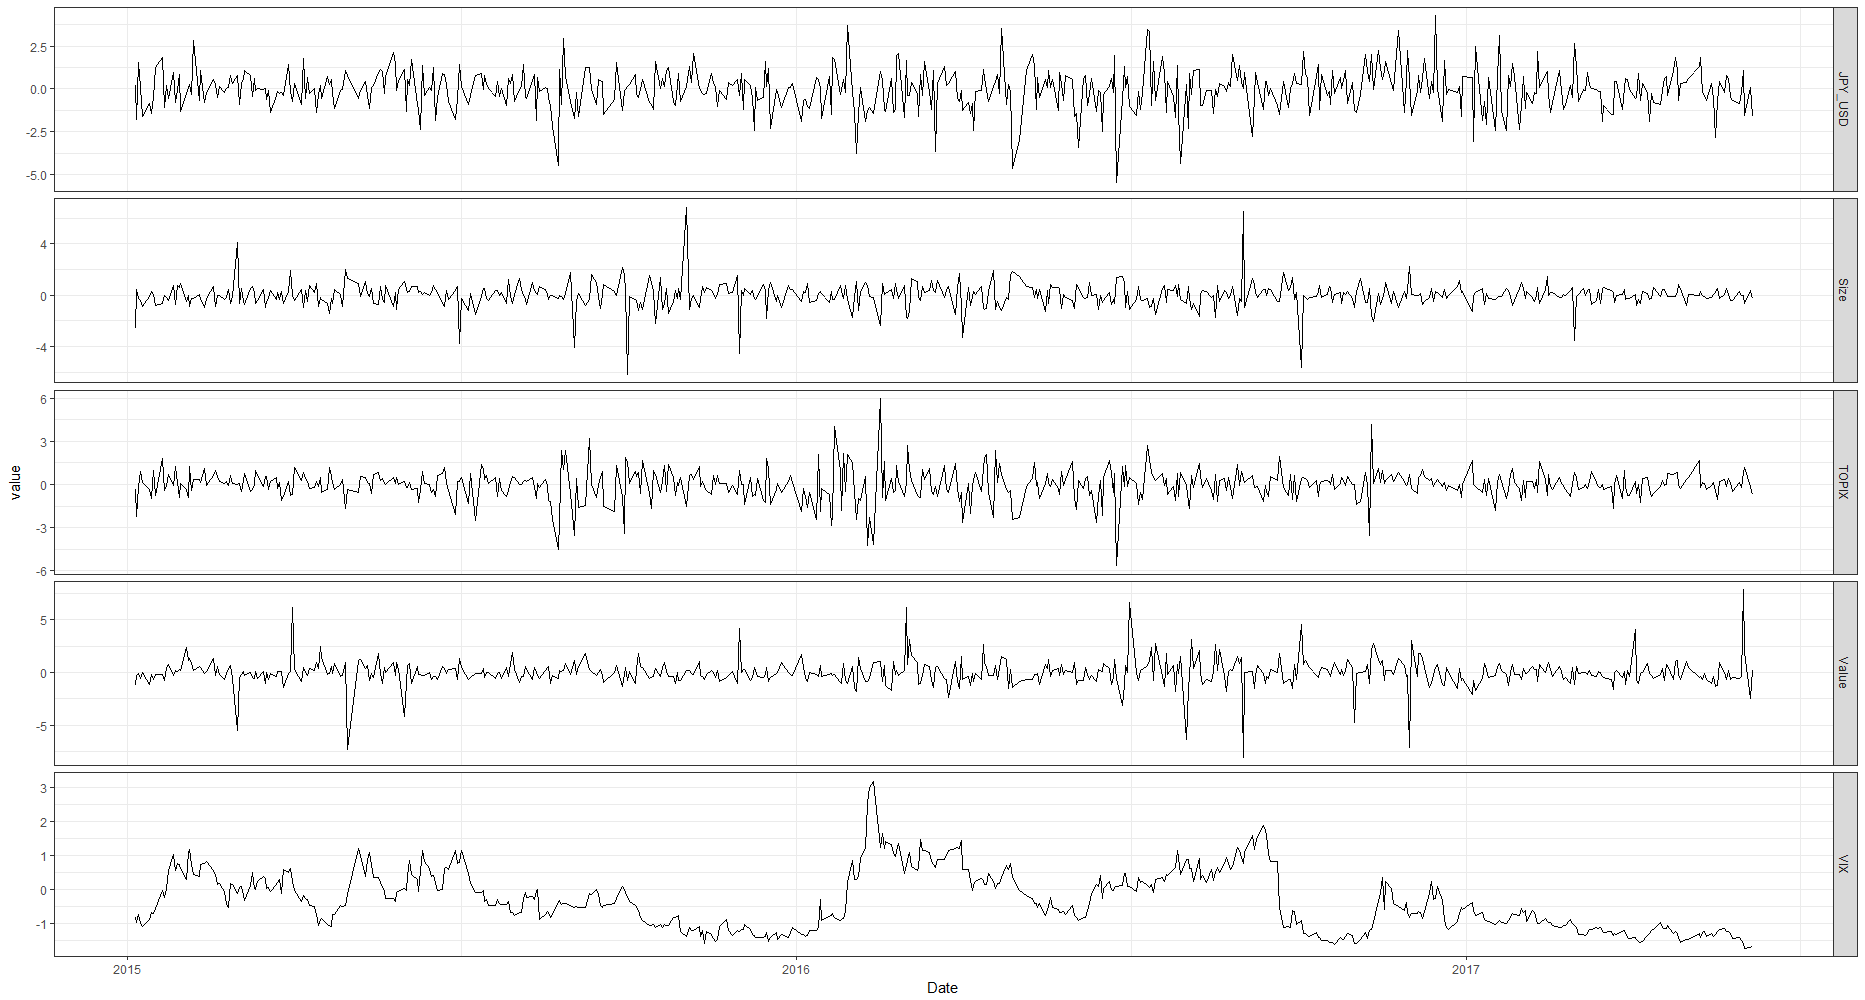
\includegraphics[width=15cm]{./fig/factor_plot.png}
		\caption{ファクターの時系列プロット}
		\label{fig:factor_plot}
	\end{center}
\end{figure}

\begin{figure}[H]
	\begin{center}
		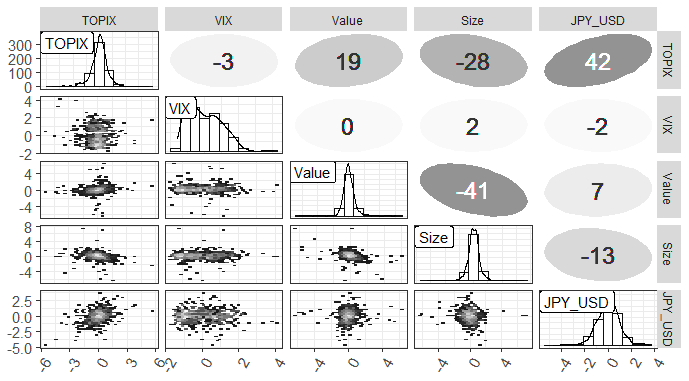
\includegraphics[width=15cm]{./fig/factor_cor.png}
		\caption{ファクター間の関係}
		\label{fig:factor_cor}
	\end{center}
\end{figure}

図\ref{fig:factor}のうちTOPIX, Value, Size, JPY$\_$USDはどれも定常のような動きになっていることが分かる。対数差分や差分を取っているこれらの系列がこのような動きを示すことは自然なことであるが、中でもValue, Sizeは時折大きな変動を見せており、従う確率分布が他とは異なる可能性がある。JPY$\_$USDの差分系列は最も変動が安定しており、TOPIXの対数差分系列がその中間ぐらいであると言える。またVIXに関してであるが、ボラティリティの大きさをファクターとして扱いたいために原系列をそのまま(差分などを取らずに)正規化した。そのため明らかに非定常過程になっており、直近半年ほどは非常に低い値をとっていることが分かる。

次に図\ref{fig:factor_cor}を確認する。既に述べたがTOPIX, Value, Sizeは時折大きな変動を見せるため、中心付近で高く裾の広い分布になっている。このことはTOPIX, Value, Size同士の散布図が中心付近に集まっており、十字型の広がりを持つことからも確認できる。図\ref{fig:factor_cor}右上の、ファクター間の相関係数を100倍した数値を確認すると、全体的に低くまとまっているものの、低い相関を持つファクターの組み合わせが存在することが見て取れる。この場合TOPIXとJPY$\_$USD、ValueとSize、TOPIXとSizeである。相関を持つ説明変数を使用しての回帰を行うといわゆる「多重共線性」の問題が発生し、実際以上に決定係数が大きくなってしまうなどの不都合がある。よってファクター全てを使ってのモデル推定は不適当であると考えられ、次節で述べるように、モデルの推定方法に工夫を施す必要がある。
%%%%%%%%%%%どうなの!?!?問題アリ???

\section{ファクターモデルの推定}
手に入れやすく扱いやすい日次終値データを対象としていることに加え,時系列データの性質により,推定するパラメータ数に対し十分な標本が得られないという問題がある.
また市場の性質が不変であるとは考えにくく,ゆるやか(もしくは何らかの偶発的なショックにより急激に)変化していくものと思われる.
そのためバックテストも見据え,3カ月分のデータを用いてモデルを推定し,その先1カ月を対象にバックテストを行うこととした.
%3カ月分のデータを使う具体的な理由があれば欲しい

マルチ・ファクターモデルを推定する際,Fama-Frenchの3ファクターモデルやCarhartの4ファクターモデルのような線形モデルだけでなく,非線形モデルも考慮に入れることができる.しかしながら,標本の少なさや時系列データにおける外挿の問題により複雑なモデルを考えるメリット小さく,ここでは線形モデルのみを考えた.

線形でのマルチ・ファクターモデルを推定する際にも注意しなければならないことがある.むやみに説明変数(ここでは各ファクターを指す)を増やすことにより生じる多重共線性の問題や多重性の問題,みせかけの回帰の問題である.そこで,説明変数を全て使用しての線形回帰ではなく,何らかの工夫を施すことによりむやみにモデルを複雑にしない操作が必要になる.選択肢としては以下の手法が考えられる.

\begin{itemize}
\item AICやBICなどの情報量基準を用いたモデル選択
\item リッジ回帰やlasso回帰などの,正則化項を用いたモデル推定
\item 介入効果と回帰係数を一致させるための統計的因果推論に基づいた説明変数選択
\end{itemize}

\subsection{lasso回帰について}
\section{リスク・プレミアム}
過去3ヶ月のデータより推定したマルチ・ファクターモデルに基づいて算出したリスク・プレミアムを以下の図\ref{fig:riskpremium}に示した。具体的には,2.6節の式(\ref{eq:fp})を一般化逆行列を利用することによりファクター・ポートフォリオを推定し,その期待超過収益率をファクターのリスク・プレミアムとした.

\begin{figure}[H]
	\begin{center}
		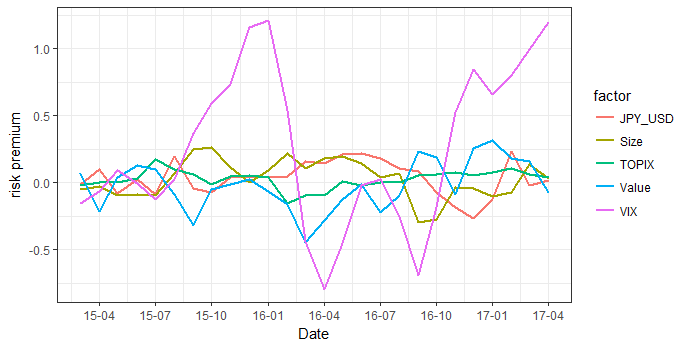
\includegraphics[width=15cm]{./fig/riskpremium.png}
		\caption{リスク・プレミアムの推移}
		\label{fig:riskpremium}
	\end{center}
\end{figure}
\section{バックテスト}
様々なポートフォリオ

\section{ポートフォリオ選択}
リスク・プレミアムを算出したことによりファクターごとのリスクを取る価値が定量化できたが、ポートフォリオの構成銘柄は10$\sim$30銘柄でなくてはならない。銘柄数を考慮しなければ、リスクプレミアムの合計を目的関数とした最適化問題を考えればよいことになる。

ポートフォリオの収益率ファクターに対する感度は2.2節の式(\ref{eq:multi})により与えられていた。今回は5ファクターモデルを考えているため、ポートフォリオの収益は次のように与えられる。
\begin{equation}
\begin{split}
R_P &= \alpha_P + \beta_{P,1} F_1 + \beta_{P,2} F_2 + \cdots + \beta_{P,5} F_m + \varepsilon_P\\
&=\sum_{i=1}^N \alpha_i + F_1 \sum_{i=1}^N w_i \beta_{i,1} + \cdots + F_5 \sum_{i=1}^N w_i \beta_{i,m} + \sum_{i=1}^N w_i\varepsilon_i\\
&= \sum_{i=1}^N \alpha_i + \sum_{k=1}^5 \sum_{i=1}^N w_i \beta_{i,k} F_k + \sum_{i=1}^N w_i\varepsilon_i
\label{eq:port}
\end{split}
\end{equation}
いま、ファクター$F_1,\cdots,F_5$のリスク・プレミアムが$\lambda_1,\cdots,\lambda_5$で与えられているとすると、ファクターのリスク・プレミアムを重みとした以下の最適化問題を考えるのが自然である。

\begin{equation}
\begin{split}
\text{maximize : }\quad & \beta_{P,1}\lambda_1 + \beta_{P,2}\lambda_2 + \beta_{P,3}\lambda_3 + \beta_{P,4}\lambda_4 + \beta_{P,5}\lambda_5\\
& = \sum_{k=1}^5 \sum_{i=1}^N w_i \beta_{i,k} F_k\\
\text{subject to : }\quad & \sum_{i=1}^N w_i = 1\\
& w_i \geq 0\qquad(i=1,\cdots,N)
\end{split}
\label{eq:port_optim}
\end{equation}
式(\ref{eq:port_optim})の最適化問題のうち、$F_k, \beta_{i,k}$は推定済みであり、$w_i$のみが変数である。よってこれは線形計画問題とな
り、シンプレックス法などのアルゴリズムにより簡単に解くことができる。

次に銘柄数を考慮する。10$\sim$30銘柄に絞り込まなければならないので、銘柄$i$がポートフォリオに組み込まれた場合に1を,そうでない場合は0を示す変数$x_i$を導入することで以下のように定式化できる。

\begin{equation}
\begin{split}
\text{maximize : }\quad & \beta_{P,1}\lambda_1 + \beta_{P,2}\lambda_2 + \beta_{P,3}\lambda_3 + \beta_{P,4}\lambda_4 + \beta_{P,5}\lambda_5\\
& = \sum_{k=1}^5 \sum_{i=1}^N w_i \beta_{i,k} \lambda_k\\
\text{subject to : }\quad & \sum_{i=1}^N w_i = 1\\
& w_i \geq 0\qquad(i=1,\cdots,N)\\
&10 \leq \sum_{i=1}^Nx_i \leq 30
\end{split}
\label{eq:port_optim}
\end{equation}

最後の式が加わったことにより,厳密解を求めることは非常に難しくなった.そこで,特定の最適化問題に依存しないメタ・ヒューリスティクスによる解法が考えられるが,計算量が多く,全ての期間でのバックテストが間に合わなかった.そのため,以下の手法によるポートフォリオ選択を考えた.

\begin{itembox}[l]{ポートフォリオ選択の手順}
\begin{enumerate}
\item 直近3ヶ月のデータより推定したファクターごとのリスク・プレミアムのうち、最もプレミアムの大きいファクターへの感度が高いもの上位100銘柄を選択する。
\item 1で選択した100銘柄のうち、直近3ヶ月のモメンタムが高い30銘柄を選択
\item 2で選択した30銘柄により等加重ポートフォリオを構成
\end{enumerate}
\end{itembox}

\chapter{途中経過}
\section{提出したポートフォリオ}

\begin{table}[H]
\begin{center}
\begin{tabular}{|c|c|c|}
\hline
企業名 & ウェート(\%) & 時価総額(円, 7月3日時点)\\
\hline
\hline
グローブライド	&3.34&3,343,642\\
コメダホールディングス&3.33	&3,335,200\\
ゼンショーホールディングス&3.33&	3,339,875\\
三井ホーム&3.33&3,333,333\\
井筒屋&3.33	&3,341,014\\
日成ビルド工業&3.35&3,360,302\\
美津濃&3.28	&3,287,108\\
藤倉ゴム工業	&	3.36	&	3,369,011	\\
近鉄百貨店	&	3.35	&	3,352,435	\\
GSIクレオス	&	3.30	&	3,309,523	\\
イマジカ・ロボット・ホールディングス	&	3.34	&3,351,877\\
グランディハウス	&	3.30	&	3,309,859	\\
サンフロンティア不動産	&	3.43	&	3,432,881	\\
北陸電力	&	3.32	&	3,326,772	\\
アイ・オー・データ機器	&	3.35	&	3,360,768	\\
アドソル日進	&	3.36	&	3,363,838	\\
システムリサーチ	&	3.36	&	3,363,148	\\
ルネサスイーストン	&	3.36	&	3,367,816	\\
日本電波工業	&	3.36	&	3,363,984	\\
ソフトクリエイトホールディングス	&	3.35	&3,361,324\\
カワチ薬品	&	3.35	&	3,353,240	\\
三井製糖	&	3.39	&	3,395,734	\\
六甲バター	&	3.30	&	3,305,533	\\
森永乳業	&	3.23	&	3,234,511	\\
養命酒製造	&	3.31	&	3,317,285	\\
ニチハ	&	3.34	&	3,350,168	\\
三井住友建設	&	3.30	&	3,306,233	\\
太平洋興発	&	3.33	&	3,333,333	\\
極東証券	&	3.28	&	3,285,697	\\
SOMPOホールディングス	&	3.35	&	3,353,441\\
\hline
\hline
合計& 100.00 &  100,208,884\\
\hline
\end{tabular}
\end{center}
\caption{提出したポートフォリオ}
\label{tbl:port1}
\end{table}
\section{7月中のパフォーマンス}
\chapter{課題とリバランス}
\section{課題}
1回目のポートフォリオ提出に間に合わなかった分析や、提出後に浮かんできた疑問点、考えうる批判など数々の課題がある。ここではそれらを列挙し、考察していく。
\subsection{リスク・プレミアム算出後のポートフォリオ選択に関して}

\end{document}